\documentclass[12pt]{article}
\usepackage{preamble2}

\title{Slopes of Perpendicular Lines}
\author{Patrick Toche}
\date{25 June 2020}

\begin{document}
\begin{minipage}{\textwidth}
\maketitle
\begin{abstract}
In a cartesian coordinate system, a line has slope $a$. Can you calculate the slope of a perpendicular line? Or is more information needed?
\end{abstract}
\end{minipage}

\section*{Slopes of Perpendicular Lines}
In a Cartesian coordinate system, a line has slope $a$. Can you calculate the slope of a perpendicular line? Or is more information needed? [In mathematics, perpendicular lines are more commonly called orthogonal lines. In the plane, the two concepts are equivalent. Orthogonality is an extension of perpendicularity to spaces of higher dimension than the plane] The situation is depicted in Figure~\ref{fig:slopes:01}:
\begin{figure}[hpbt]
\begin{minipage}[b]{\textwidth}
\centering
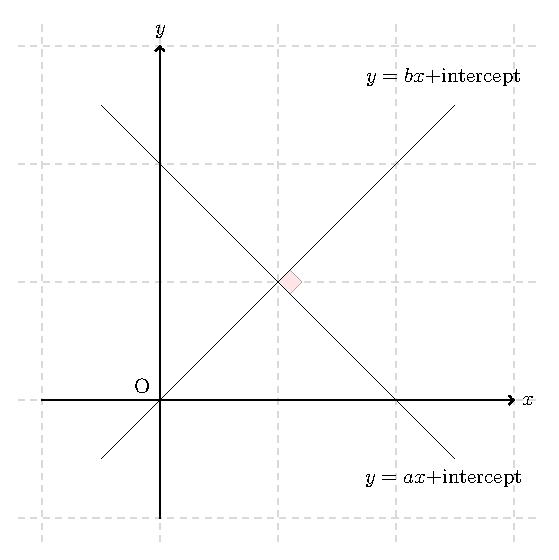
\includegraphics[width=0.6\textwidth]
{coordinates-and-slopes-1}
\caption{\textbf{Two Orthogonal Lines in a Cartesian Coordinate System}. 
\label{fig:slopes:01}}
\end{minipage}
\end{figure}

We have very little information to go by. Can we infer the slope $b$ from $a$? Note that since only the slope matters in this problem, we can consider two lines that intersect at the origin. Figure~\ref{fig:slopes:02} shows that we can also represent the slopes graphically. As we are now considering two lines that intersect at the origin, their equations are simply $y=ax$ and $y=bx$. And so for $x=1$, say, we have $y=a$ on line $OA$ and $y=b$ on line $OB$. Can we find an expression for $b$ in terms of $a$? Yes, by considering several right triangles and applying the Pythagoras theorem.
\begin{figure}[hpbt]
\begin{minipage}[b]{\textwidth}
\centering
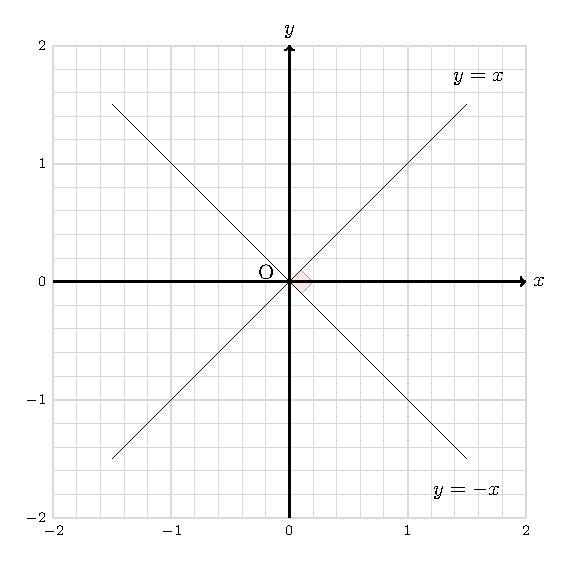
\includegraphics[width=0.6\textwidth]
{coordinates-and-slopes-2}
\caption{\textbf{Two Orthogonal Lines form Three Pythagorean Triangles}. 
\label{fig:slopes:02}}
\end{minipage}
\end{figure}

Triangle $AOB$ yields:
\begin{align*}
(b-a)^2 = OA^2 + OB^2
\end{align*}

Triangle $OaA$ yields:
\begin{align*}
OA^2 = 1^2 + a^2
\end{align*}

Triangle $ObB$ yields:
\begin{align*}
OB^2 = 1^2 + b^2
\end{align*}

Putting it all together gives:
\begin{align*}
(b-a)^2 
  & = ~OA^2~~~ + ~~~OB^2 \\
  & = 1^2 + a^2 ~+~ 1^2 + b^2 \\
b^2 - 2ab + a^2 
  & = a^2 + b^2 + 2 \\
-2ab & = 2\\
b & = -\frac{1}{a}
\end{align*}

The slope of any perpendicular line is therefore equal to the opposite of the inverse slope --- or minus the inverse: \fbox{$b = -1/a$}. The special case $a=1$ (the $45^\circ$ degree line) is well known. 
\end{document}